%% Commands for TeXCount
%TC:macro \cite [option:text,text]
%TC:macro \citep [option:text,text]
%TC:macro \citet [option:text,text]
%TC:envir table 0 1
%TC:envir table* 0 1
%TC:envir tabular [ignore] word
%TC:envir displaymath 0 word
%TC:envir math 0 word
%TC:envir comment 0 0
%%
%% The first command in your LaTeX source must be the \documentclass
%% command.
%%
%% For submission and review of your manuscript please change the
%% command to \documentclass[manuscript, screen, review]{acmart}.
%%
%% When submitting camera ready or to TAPS, please change the command
%% to \documentclass[sigconf]{acmart} or whichever template is required
%% for your publication.
%%
%%
\documentclass[sigconf, screen]{acmart}
%%
%% \BibTeX command to typeset BibTeX logo in the docs
\AtBeginDocument{%
  \providecommand\BibTeX{{%
    Bib\TeX}}}

%%
%% Additional packages required for this document
\usepackage{lipsum} % For generating dummy text
\usepackage{tikz}
\usetikzlibrary{arrows.meta, positioning, fit, backgrounds, matrix}

%% Rights management information.  This information is sent to you
%% when you complete the rights form.  These commands have SAMPLE
%% values in them; it is your responsibility as an author to replace
%% the commands and values with those provided to you when you
%% complete the rights form.
\setcopyright{acmlicensed}
\copyrightyear{2025}
\acmYear{2025}
\acmDOI{XXXXXXX.XXXXXXX}
%% These commands are for a PROCEEDINGS abstract or paper.
\acmConference[RTKS '25]{Real-Time Kernels and Systems Exam}{Fill in Date}{Padova, Italy}
%%
%%  Uncomment \acmBooktitle if the title of the proceedings is different
%%  from ``Proceedings of ...''!
%%
%%\acmBooktitle{Woodstock '18: ACM Symposium on Neural Gaze Detection,
%%  June 03--05, 2018, Woodstock, NY}
\acmISBN{978-1-4503-XXXX-X/2018/06}


%%
%% Submission ID.
%% Use this when submitting an article to a sponsored event. You'll
%% receive a unique submission ID from the organizers
%% of the event, and this ID should be used as the parameter to this command.
%%\acmSubmissionID{123-A56-BU3}

%%
%% For managing citations, it is recommended to use bibliography
%% files in BibTeX format.
%%
%% You can then either use BibTeX with the ACM-Reference-Format style,
%% or BibLaTeX with the acmnumeric or acmauthoryear sytles, that include
%% support for advanced citation of software artefact from the
%% biblatex-software package, also separately available on CTAN.
%%
%% Look at the sample-*-biblatex.tex files for templates showcasing
%% the biblatex styles.
%%

%%
%% The majority of ACM publications use numbered citations and
%% references.  The command \citestyle{authoryear} switches to the
%% "author year" style.
%%
%% If you are preparing content for an event
%% sponsored by ACM SIGGRAPH, you must use the "author year" style of
%% citations and references.
%% Uncommenting
%% the next command will enable that style.
%%\citestyle{acmauthoryear}


%%
%% end of the preamble, start of the body of the document source.
\begin{document}

%%
%% The "title" command has an optional parameter,
%% allowing the author to define a "short title" to be used in page headers.
\title{Analysis and Implementation of a Real-Time Demonstrator on the RTIC Runtime}

%%
%% The "author" command and its associated commands are used to define
%% the authors and their affiliations.
%% Of note is the shared affiliation of the first two authors, and the
%% "authornote" and "authornotemark" commands
%% used to denote shared contribution to the research.
\author{Gianluca Bresolin}
\email{gianluca.bresolin@studenti.unipd.it}
\affiliation{%
  \institution{Università degli Studi di Padova}
  \city{Padova}
  \state{Veneto}
  \country{Italy}
}

\author{Tommaso Prandin}
\email{tommaso.prandin@studenti.unipd.it}
\affiliation{%
  \institution{Università degli Studi di Padova}
  \city{Padova}
  \state{Veneto}
  \country{Italy}
}

%%
%% By default, the full list of authors will be used in the page
%% headers. Often, this list is too long, and will overlap
%% other information printed in the page headers. This command allows
%% the author to define a more concise list
%% of authors' names for this purpose.
%\renewcommand{\shortauthors}{Trovato et al.}

%%
%% The abstract is a short summary of the work to be presented in the
%% article.
\begin{abstract}
  This paper presents the implementation and analysis of a real-time
  demonstrator originally developed in \textit{Ada} using the \textit{Ravenscar
  Profile}, re-implemented in \textit{Rust} using the \textit{RTIC} framework.  
  The demonstrator is designed to run on an \textit{STM32F4} microcontroller and
  uses a \textit{Fixed-Priority Scheduling} policy combined with \textit{Stack
  Resource Policy (SRP)} for resource sharing. 
  The analysis is performed using the \textit{MAST} tool to verify timing
  properties and analyze system performance under various workloads.   
  The results demonstrate the feasibility of adopting \textit{Rust} and
  \textit{RTIC} for real-time applications, while also highlighting differences 
  and considerations compared to the original \textit{Ada} implementation.
\end{abstract}

%%
%% The code below is generated by the tool at http://dl.acm.org/ccs.cfm.
%% Please copy and paste the code instead of the example below.
%%
\begin{CCSXML}
<ccs2012>
   <concept>
       <concept_id>10011007.10010940.10010971.10011679</concept_id>
       <concept_desc>Software and its engineering~Real-time systems software</concept_desc>
       <concept_significance>500</concept_significance>
       </concept>
   <concept>
       <concept_id>10011007.10010940.10010971.10010564</concept_id>
       <concept_desc>Software and its engineering~Embedded software</concept_desc>
       <concept_significance>500</concept_significance>
       </concept>
   <concept>
       <concept_id>10011007.10010940.10010971.10010972</concept_id>
       <concept_desc>Software and its engineering~Software architectures</concept_desc>
       <concept_significance>300</concept_significance>
       </concept>
 </ccs2012>
\end{CCSXML}

\ccsdesc[500]{Software and its engineering~Real-time systems software}
\ccsdesc[500]{Software and its engineering~Embedded software}
\ccsdesc[300]{Software and its engineering~Software architectures}

%%
%% Keywords. The author(s) should pick words that accurately describe
%% the work being presented. Separate the keywords with commas.
\keywords{Real-Time Kernels, Real-Time Systems, Embedded Software, Software Architectures}
%% A "teaser" image appears between the author and affiliation
%% information and the body of the document, and typically spans the
%% page.
% \begin{teaserfigure}
%   \includegraphics[width=\textwidth]{example-image-a}
%   \caption{Caption}
%   \Description{Enjoying the baseball game from the third-base
%   seats. Ichiro Suzuki preparing to bat.}
%   \label{fig:teaser}
% \end{teaserfigure}

% \received{20 September 2025}
% \received[revised]{}
% \received[accepted]{}

%%
%% This command processes the author and affiliation and title
%% information and builds the first part of the formatted document.
\maketitle

\section{Introduction}
Real-time embedded systems demand precise control over timing, concurrency and
resource management.  
Such systems are often used in critical applications where failure to meet
timing constraints can lead to severe consequences. Hence, developing a
real-time system requires careful consideration of the underlying runtime
environment, necessitating a clear understanding of how the system will behave
in order to provide sufficient guarantees on meeting timing requirements. \\
The choice of the runtime environment is a crucial aspect in the design of a
real-time system, as it can significantly impact the system's ability to meet
its desired behaviour through reliable mechanisms it offers. One of the most
popular languages that meets the needs of real-time systems is \textit{Ada},
which has been widely used in the development of safety-critical systems due to
its deterministic constructs that allow high analysability of the code. While
\textit{Ada} remains a robust choice, recent advances in the \textit{Rust}
programming language have introduced new opportunities for real-time systems
development. \\ 
In this paper, a real-time system originally implemented using the \textit{Ada
Ravenscar Profile} is re-implemented in \textit{Rust} using the\textit{Real-Time
Intrupput-driven Concurrency (RTIC)} framework, which is responsible for
managing the scheduling of tasks through a \textit{Fixed-Priority Scheduling}
and the resource sharing in the system under \textit{Stack Resource Policy
(SRP)}. \\ 
For the analysis of the system, the \textit{MAST} tool is used to verify the
timing properties and to analyze the system under different workloads, which is
run on a \textit{STM32F4} microcontroller. \\ 
The goal of this work is to demonstrate the feasibility of using Rust and RTIC
for real-time systems, while also providing some considerations and comparison
with the original \textit{Ada} implementation. \\ 
The rest of the paper is organized as follows. Section 2 presents a formal
description of the system model. Section 3 introduces the \textit{RTIC}
framework and its key concepts. Sections 4 and 5 discuss the measurement of
execution times and the detection of deadline misses, respectively. Section 6
provides an overview of the \textit{MAST} tool and its analysis capabilities. In
Section 7, we present the \textit{Fixed-Priority Scheduling (FPS)} analysis of
the system. Finally, Section 8 concludes the paper reporting the main findings.  

\section{System Model}
The software architecture follows the one proposed in "\textit{Guide for the Use
of Ada Ravenscar Profile in High Integrity Systems}"
\cite{burnsGuideUseAda2004}. It is comprised by one periodic producer task that
can activate two other sporadic tasks. Additionally, there is a sporadic event
server that manages the occurrence of external events. In the implemented
application events are generated by a periodic task that emulate user
interaction, for repeatability reasons. 

Table [\ref{tab:tasks-list}] contains the list of tasks constituting the
application, together with their typology, deadline, period (if applicable) and
priority. Priorities have been assigned using the \textit{Deadline Monotonic}
algorithm, which assigns priorities in decreasing order, starting with jobs of
smaller relative deadline. It is an optimal algorithm for constrained deadlines
and fixed-priority scheduling \cite[p.~119]{liuRealTimeSystems2000}. \\ 
The deadline watchdogs have been given the highest priority in order to detect
overrun without interference from other tasks (see section
\ref{sec:DeadlineMissDetection} for furhter details).

The tasks in the system share various resources. Access is regulated by variants
of the \textit{Priority Ceiling Protocol}
\cite{shaPriorityInheritanceProtocols1990} depending on the implementation: the
Ada system implements the \textit{Immediate Priority Ceiling Protocol}
\cite{chengImplementationPriorityCeiling2007}, while the Rust system uses
\textit{Stack Resource Policy} \cite{bakerStackbasedSchedulingRealtime1991}.\\ 
While the implementation is slightly different, both protocols show the same
properties and response-time behavior. They require to specify the ceiling value
for each shared resource, which is obtained by picking the maximum priority
value among all the task using the given resource. 

Table [\ref{tab:res-list}] contains the list of all the shared resources in the
system, together with their users (tasks) and their priority ceiling. 

\begin{table*}[!t]
  \centering
    \begin{tabular}{p{0.2\linewidth} p{0.2\linewidth} p{0.1\linewidth}
    p{0.2\linewidth} p{0.1\linewidth}}
      \hline
        \textbf{Task} & \textbf{Task Type} & \textbf{Period (ms)} & 
        \textbf{Deadline (ms)} & \textbf{Priority} \\
      \hline
        Activation Log Reader & Sporadic & 3000 & 1000 & 3\\
        On Call Producer & Sporadic & 5000 & 800 & 5 \\
        Regular Producer & Periodic & 1000 & 500 & 7 \\
        External Event Server & Sporadic (interrupt) & 5000 & 100 & 11 \\
        Interrupt Generator & Periodic & 5000 & 50 & 13 \\
        ALR Deadline Watchdog & Sporadic & 3000 & 1000 & 15 \\
        OCP Deadline Watchdog  & Sporadic & 5000 & 800 & 15 \\
        RP Deadline Watchdog & Periodic & 1000 & 500 & 15 \\
        EES Deadline Watchdog & Sporadic (interrupt) & 5000 & 100 & 15 \\
      \hline
    \end{tabular}
  \caption[Task Table]{List of tasks in the system, with their parameters}
  \label{tab:tasks-list}
\end{table*}

\begin{table*}[!t]
  \centering
  \begin{tabular}{ p{0.2\linewidth} p{0.5\linewidth} p{0.1\linewidth}}
    \hline
    \textbf{Resource} & \textbf{Users} & \textbf{Ceiling}\boldmath{$\pi_R$} \\
    \hline
    Activation Log & Activation Log Reader, External Event Server & 11 \\
    Event Queue & External Event Server, External Event ISR & 11 \\
    Request Buffer & Regular Producer, On-Call Producer & 7 \\
    ALR Deadline Object & Activation Log Reader, ALR Deadline Watchdog & 15 \\
    OCP Deadline Object & On-Call Producer, OCP Deadline Watchdog & 15 \\
    RP Deadline Object & Regular Producer, RP Deadline Watchdog & 15 \\
    EES Deadline Object & External Event Server, EES Deadline Watchdog & 15 \\
    \hline  
  \end{tabular}
  \caption[Resource table]{List of shared resources in the system, with their 
  users and priority ceilings} 
  \label{tab:res-list}
\end{table*}

In order to emulate a realistic workload for task requiring some kind of
computation, the small variant of the Whetstone benchmark
\cite{curnowSyntheticBenchmark1976} is used. It includes different kind of
computations: integer, floating-point, trigonometry, branches and function
calls, with the aim of testing the system under a wide range of loads. \\ 
This workload is a parameter that we used in the analysis section to create
different workload levels and observe the resulting behavior of the system,
first by simulating it using the MAST tool \cite{MASTComprehensiveTool}, then by
running the application in a real setting.

To this end, we have used the \textit{Olimex STM32\-H405} \cite{olimexSTM32H405}
development board, together with a \textit{STLink\-v2} \cite{STLINKV2Tool}
debugging probe. 

\subsection{Tasks Description}

\subsubsection{Activation Log Reader}

The \textit{Activation Log Reader} is a sporadic task which awaits on a signal
received from the \textit{Regular Producer}, and then performs its internal
operation which consists of an artificial Whetstone workload, followed by a
reading of the status of the \textit{Activation Log} and a print that notifies
the end of its sporadic activation.

\subsubsection{On-Call Producer}

The \textit{On-Call Producer} is a sporadic task that waits for a request
deposit into the \textit{Request Buffer}, then reads it and runs a Whetstone
workload with load equal to the extracted value. The requests are sent by the
\textit{Regular Producer}, and they are meant to represent a scenario in which a
main task delegates some work to a helper task in the event of an overload. 

\subsubsection{Regular Producer}

The \textit{Regular Producer} is a periodic task that runs a Whetstone workload
with a predefined load value, then, based on a predetermined criterion, can
release the \textit{Activation Log Reader} and send a work request to the
\textit{On-Call Producer}. 

\subsubsection{External Event Server}

The \textit{External Event Server} is a sporadic task that waits for events put
onto the \textit{Event Queue} by the interrupt handler bound to the simulated
external event. It updates the \textit{Activation Log} counter on each
activation. 

\subsubsection{Deadline Watchdogs}

For every task in the system there is a watchdog monitor task that checks for
deadline overruns. It has the maximum priority to prevent interference. It
maintains the number of deadline misses and whenever it detects one 
it prints a warning message (see section \ref{sec:DeadlineMissDetection} for
further details). \\

\noindent Figure [\ref{fig:system-architecture}] shows a high-level view of the system
architecture 

\begin{figure}[t]
  \centering
  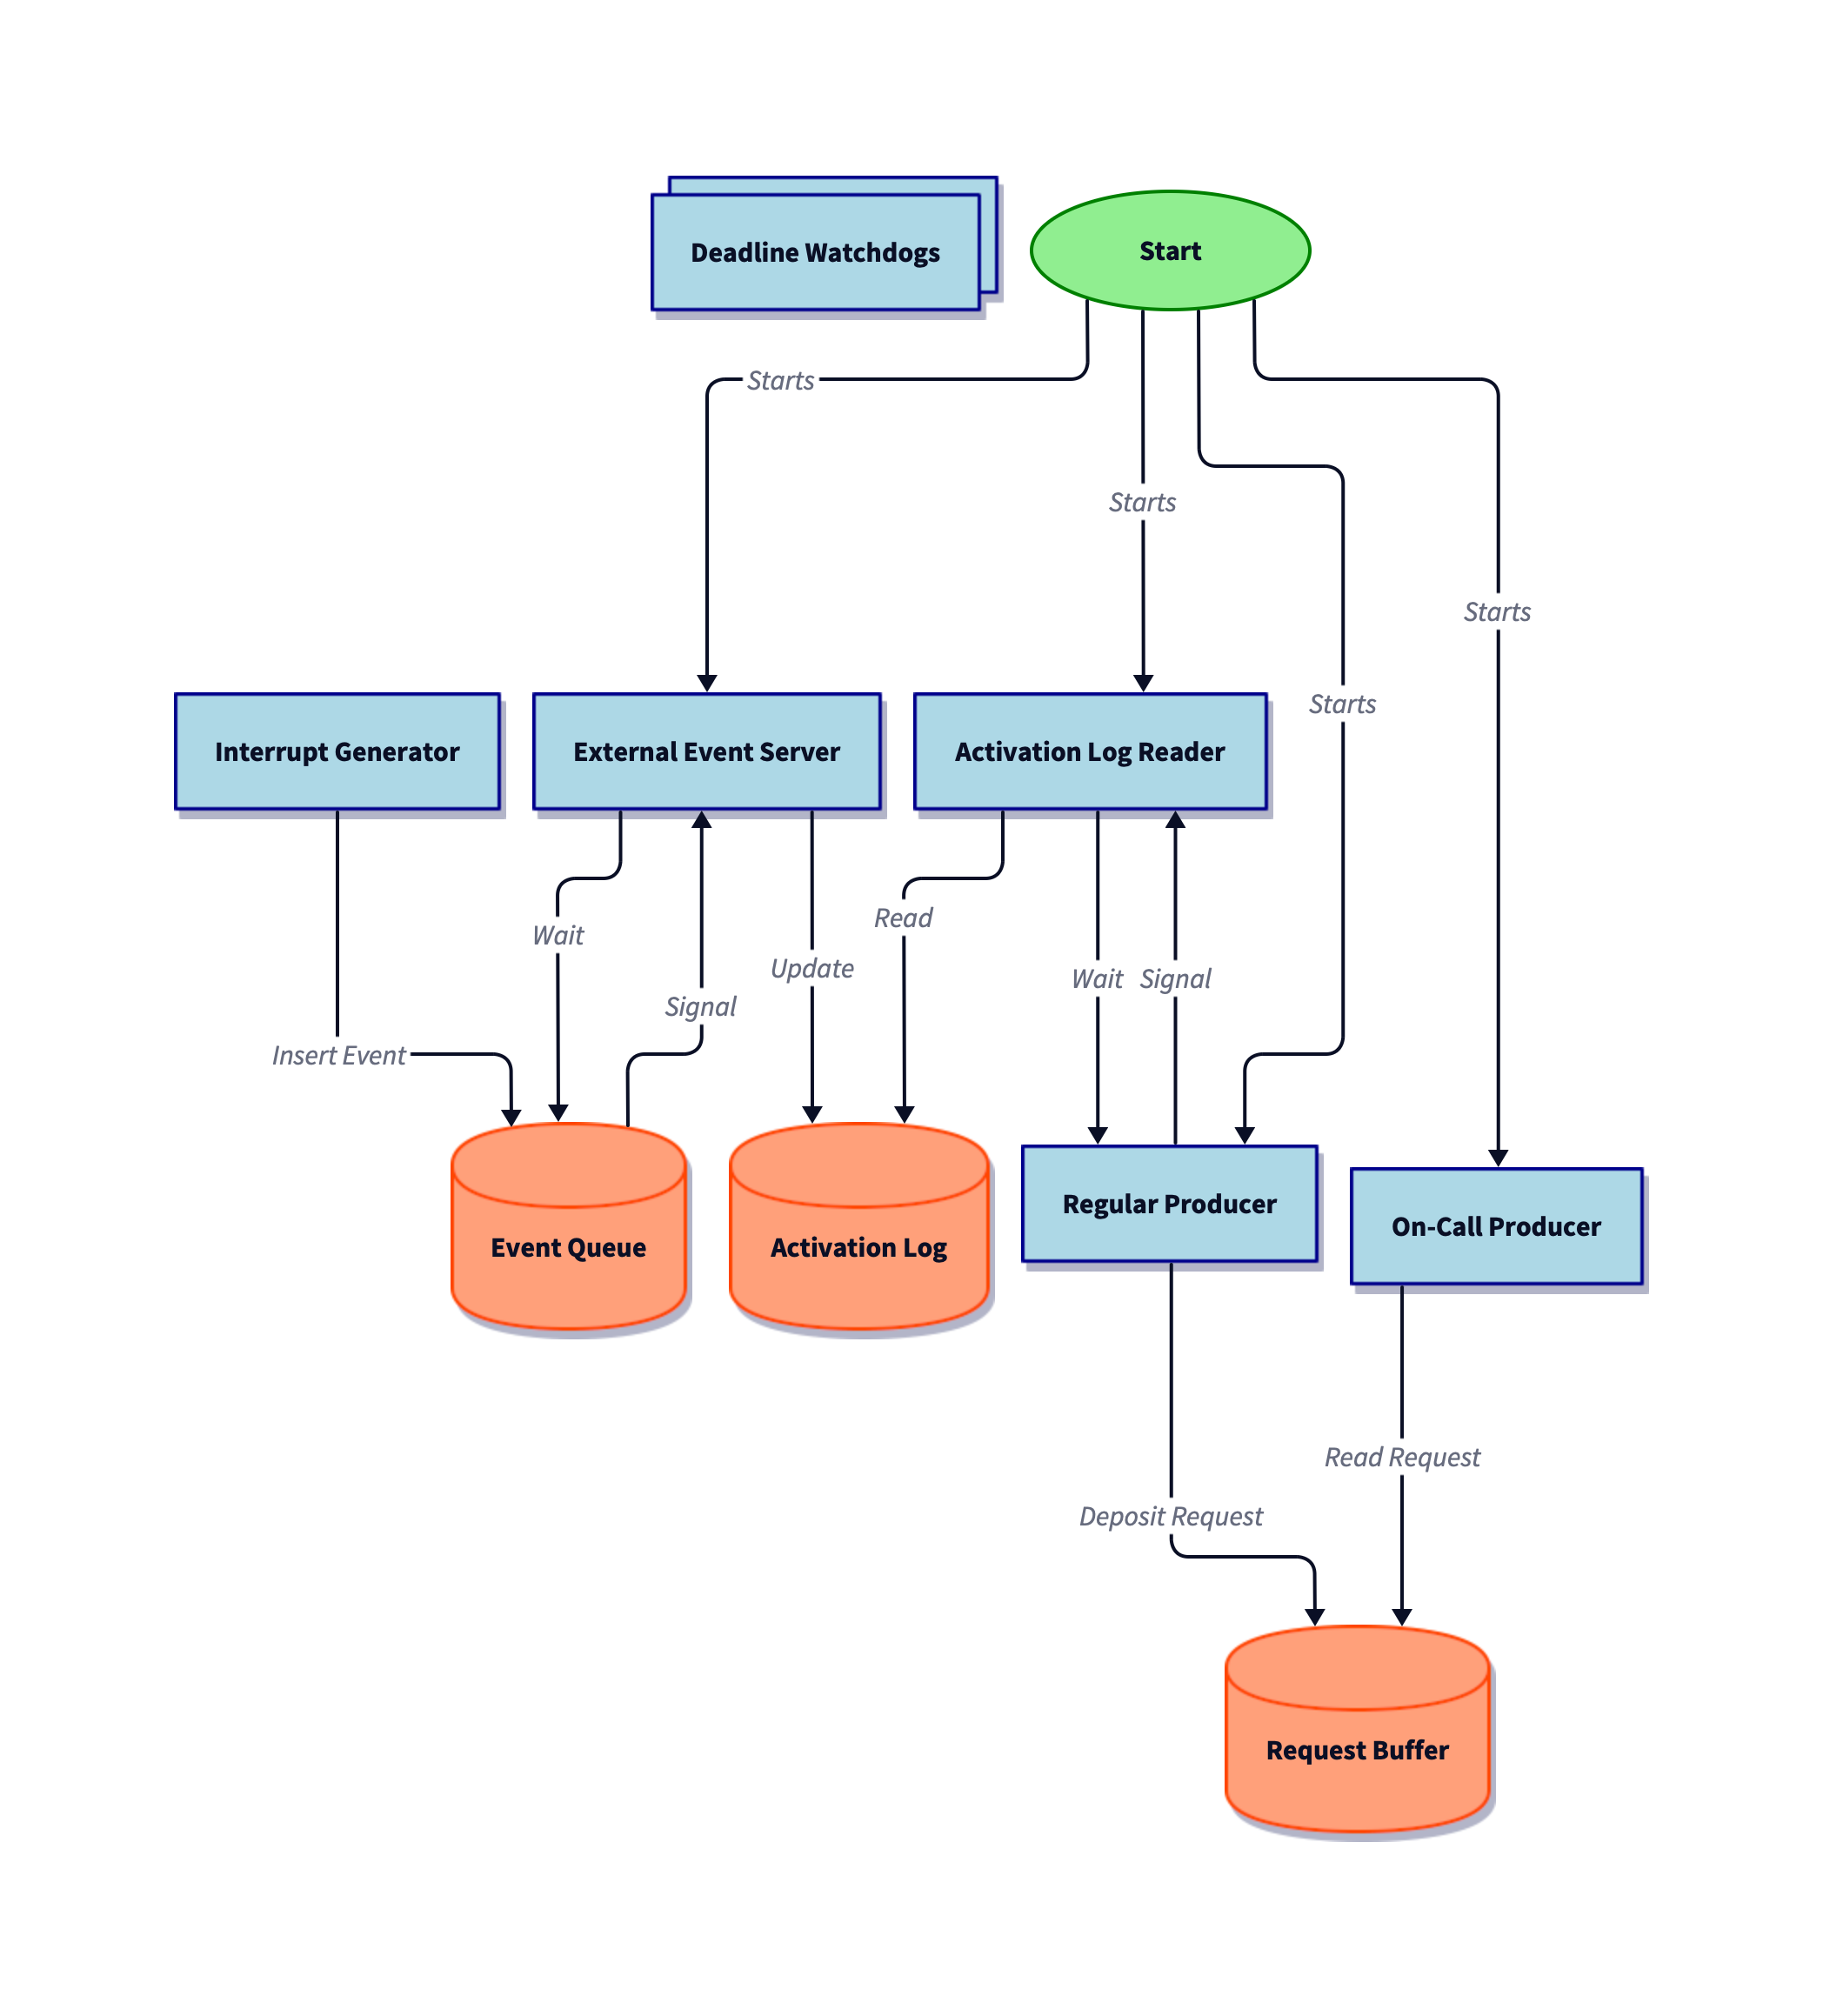
\includegraphics[width=0.45\textwidth]{images/system-diagram.png}
  \caption[System architecture]{System architecture diagram}
  \label{fig:system-architecture}
\end{figure}

\input{sections/rtic.tex}

\section{Execution Times}

\subsection{Rust}

Obtaining the \textit{Worst-Case Execution Times} for every operation in the
system is a crucial step in order to perform response-time analysis. 

We decided to leverage the \textit{Data Watchpoint and Trace Unit (DWT)}
\cite[Chapter~9]{armlimitedARMCortexM42009}. \textit{DWT} supports multiple
functionalities such as: debugger hardware watchpoints, multiple comparators,
and cycle counters. For our purposes, the latter one was sufficient. 

In particular, the \textit{DWT} peripheral holds a cycle counter that can be
read from the \texttt{DWT\_CYCCNT} register, which in turn can be used to
implement a simple \textit{stopwatch} that can measure time spans. 

The chosen \textit{HAL} \cite{Stm32rsStm32f4xxhal2025} already provides a
stopwatch implementation that correctly handles the wrap around of the clock
counter. The typical system clock frequency of our board is \unit[168]{MHz},
which makes the period $T = \frac{1}{f} \simeq \unit[5.95]{ns}$. Since the
counter size is \unit[32]{bits}, it will wrap around every $2^{32} \cdot T
\simeq \unit[25]{s}$, thus it must be handled to prevent wrong readings. 

The stopwatch implementation provides an API that closely resembles the workings
of a manual stopwatch: it exports a \texttt{reset} function that simply clears
every stored time, and a \texttt{lap} method that stores the current cycle count
into a buffer passed during initialization. Lap times can be simply obtained by
subtracting successive cycle counts, having care of handling wrap around. 

Since this implementation is really basic, we have designed a higher-level
abstraction that allows us to obtain the WCET of selected code sections,
corresponding to the operations under analysis. 
Listing [\ref{lst:profiler-abstraction}] shows the \textit{trait} definition for
our profiler abstraction. The \texttt{lap} method gets called at the end of
every iteration (i.e. job execution), using the saved laps; then results can be
logged using the corresponding method. 

Every different task gets a tailored implementation of the profiler
\textit{trait}; they mainly differ on the implementation of the
\texttt{update\_wcet} method, to accommodate the different operations inside the
tasks. 

\begin{listing}
  \begin{minted}[breaklines]{rust}
    pub trait Profiler {
      fn reset(&mut self);
      fn lap(&mut self);
      fn lap_time(&self, lap: usize) -> Option<ProfilingDuration>;
      fn update_wcet(&mut self);
      fn log(&self);
  }
  \end{minted}
  \caption[Profiler abstraction code]{Profiler trait used to extract WCET}
  \label{lst:profiler-abstraction}
\end{listing}

The profiling instrumentation is gated behind \texttt{cargo} \textit{features}:
when the user desires to start the profiling of a certain operation it needs to
enable the related feature at compile-time. This ensures that the application is
completely devoid of profiling objects and instructions that are not needed
during normal operation, improving performance and code size. 

The runtime does not provide a \textit{task time} like Ada Ravenscar, hence, to
obtain the desired WCET, we had to manually raise the priority of the task under
analysis in order to prevent any interference that could invalidate our times.
This is not a very clean solution, but implementing a proper task execution time
would require non-trivial modifications to the RTIC runtime, which were
considered out of the scope of the work and too time-consuming. Nonetheless, the
WCET obtained remain valid. 

We have decided to take the maximum execution time among one-thousand
executions; when the correct profiling feature is enabled, the tasks are
configured to automatically log the WCET results accumulated by the profiler and
then panic to stop execution. 

\subsection{Ada}

Concerning the Ada system, we have re-utilized the instrumentation implemented
by J. Hu and A. Gobbo in their work \cite{huJiayihuSRT2024}, aimed to perform
response-time analysis over the \textit{Ada} system model, as shown in the
original paper \cite{burnsGuideUseAda2004}.

\subsection{WCET Times}

This section contains the obtained WCET values. Both implementations have been
compiled in \textit{release} mode (i.e. with all optimizations enabled), and run
on the board at maximum clock speed (\unit[168]{MHz}). 

We have observed some significant differences in execution times for certain
operations between the Ada and Rust system. We ascribe these gaps to differences
in I/O backends and runtime overheads, since RTIC heavily relies on hardware
features specific to ARM Cortex architecture, to compiler choices, and different
math libraries. 

\subsubsection{Activation Log Reader}
\begin{table}[H]
  \centering
  \begin{tabular*}{\linewidth}{@{\extracolsep{\fill}}lrr@{}}
    \toprule
    \textbf{Operation} & \textbf{Rust (\unit{ns})} & \textbf{Ada (\unit{ns})} \\
    \midrule
    Small Whetstone (workload 139) & 4346391 & 1018910 \\
    AL Read & 136 & 1267 \\
    ALR Read & 647 & 3256 \\
    Put Line & 8017 & 8222 \\
    \bottomrule
  \end{tabular*}
  \caption{WCET per operation — Activation Log Reader}
  \label{tab:wcet-activation-log-reader}
\end{table}

\subsubsection{External Event Server}
\begin{table}[H]
  \centering
  \begin{tabular*}{\linewidth}{@{\extracolsep{\fill}}lrr@{}}
    \toprule
    \textbf{Operation} & \textbf{Rust (\unit{ns})} & \textbf{Ada (\unit{ns})} \\
    \midrule
    AL Write & 583 & 1678 \\
    EES Write & 1071 & 3322 \\
    \bottomrule
  \end{tabular*}
  \caption{WCET per operation — External Event Server}
  \label{tab:wcet-external-event-server}
\end{table}

\subsubsection{On-Call Producer}
\begin{table}[H]
  \centering
  \begin{tabular*}{\linewidth}{@{\extracolsep{\fill}}lrr@{}}
    \toprule
    \textbf{Operation} & \textbf{Rust (\unit{ns})} & \textbf{Ada (\unit{ns})} \\
    \midrule
    RB Extract & 303 & 1361 \\
    Extract Workload & 814 & 4760 \\
    Small Whetstone (workload 278) & 8692782 & 2037820 \\
    Put Line & 7970 & 7406 \\
    \bottomrule
  \end{tabular*}
  \caption{WCET per operation — On-Call Producer}
  \label{tab:wcet-on-call-producer}
\end{table}

\subsubsection{Regular Producer}
\begin{table}[H]
  \centering
  \begin{tabular*}{\linewidth}{@{\extracolsep{\fill}}lrr@{}}
    \toprule
    \textbf{Operation} & \textbf{Rust (\unit{ns})} & \textbf{Ada (\unit{ns})} \\
    \midrule
    Small Whetstone (workload 756) & 23639364 & 5541700 \\
    Due Activation & 214 & 1344 \\
    RB Deposit & 2398 & 3583 \\
    OCP Activation & 2903 & 5283 \\
    Check Due & 208 & 1372 \\
    ALR Signal & 1982 & 6922 \\
    Cancel Deadline & 273 & 2835 \\
    RP Cancel Deadline & 8314 & -- \\
    \bottomrule
  \end{tabular*}
  \caption{WCET per operation — Regular Producer}
  \label{tab:wcet-regular-producer}
\end{table}

\subsubsection{Kernel/Runtime Overheads}
\begin{table}[H]
  \centering
  \begin{tabular*}{\linewidth}{@{\extracolsep{\fill}}lrr@{}}
    \toprule
    \textbf{Operation} & \textbf{Rust (\unit{ns})} & \textbf{Ada (\unit{ns})} \\
    \midrule
    Systick Overhead & 702 & 3906 \\
    ISR Switch & 2732 & 2850 \\
    Delay Until & 865 & 5420 \\
    Signal RTIC & 4160 & -- \\
    Task Semaphore & 4178 & -- \\
    Event Queue & 4101 & -- \\
    Spawn Overhead & 148 & -- \\
    Context-Switch & 166 & 3090 \\
    \bottomrule
  \end{tabular*}
  \caption{WCET — Kernel/Runtime Overheads}
  \label{tab:wcet-kernel-overheads}
\end{table}


\section{Deadline Miss Detection}
In our system, each task is associated with an hard deadline, as described in
Table \ref{tab:tasks-list}. In order to detect a deadline miss, since the 
\textit{RTIC} framework does not provide any built-in mechanism for this, for
each task we implemented a watchdog task responsible for monitoring its
deadline. \\ 
To achieve the desired behaviour, i.e., a watchdog declares a deadline miss if
and only if the associated task fails to complete its execution before its
deadline, we used a shared resource, called
\texttt{deadline\_protected\_object}. This resource is a struct containing a
boolean flag, which value rappresents whether the task has completed its
execution or not. In \textit{RTIC} framework, each shared resource needs
to be acquired before being accessed or before invoking any of its associated
methods. Therefore, when a monitored task acquired the lock on the
\texttt{deadline\_protected\_object} to invoke \texttt{cancel\_deadline}, the
method responsible for acknowledging the deadline, it can not be preempeted by
its watchdog task. This prevents the watchdog from preempting the monitored task
while it is updating the flag, avoiding undesired deadline miss detections. \\
Additionaly, the \texttt{deadline\_protected\_object} struct contains an
activations counter, which allows for finer control over the requests to clear
deadline misses, allowing stale requests to be ignored. \\
Since in our system we have periodic and sporadic tasks, we implemented two
different types of watchdogs: 
\begin{itemize}
    \item \texttt{periodic\_deadline\_watchdog}: this watchdog has as locals are
    the period and the next deadline of the monitored task. It delays itself
    until the next deadline and then, after acquiring the shared
    \texttt{deadline\_protected\_object}, it invokes on it the method
    \texttt{deadline\_miss\_detected}. This method checks the flag and, if it is
    still false, it declares a deadline miss. Then, the watchdog increments the
    next deadline by the period of the monitored task and it loops again;
    \item \texttt{sporadic\_deadline\_watchdog}: this watchdog waits on an
    activation signal that notices it of a new activation of the monitored task. 
    The watchdog then calculates the next deadline by adding the relative
    deadline with the activation time of the monitored task, passed as argument
    inside the precedent signal. The watchdog then delays itself until the
    obtained absolute deadline and, after acquiring the shared
    \texttt{deadline\_protected\_object}, it invokes on it the method 
    \texttt{deadline\_miss\_detected}, as happens in the \\
    \texttt{periodic\_deadline\_watchdog} case. After that, it loops again,
    waiting for the next activation signal.
\end{itemize}
To avoid the first activation of a periodic watchdog from starting before the
monitored task can actually execute due to system initialisation, 
we set its first deadline equal to the system activation instant plus the
task's relative deadline. 
The system activation instant consists in a static \texttt{AtomicU32}
rappresenting, in ticks, the instant befoore which all initializtion-spawned
tasks are delayed: this mechanisms provides the system with a well defined
"\textit{zero time}". \\ 
Moreover, in order to provide accurate deadline management
for sporadic tasks, their activation signals occur inside a critical section.
This prevents unwanted preemptions between the task activation and the sending
of the signal to the corresponding watchdog, which could otherwise lead to an
incorrect calculation of the next deadline.  

\section{MAST}
The response time analysis of the system has been largely performed using the
\textit{MAST} tool \cite{MASTComprehensiveTool}. \textit{MAST} is a
\textit{Modeling and Analysis Suite for Real-Time} applications, developed at
the \textit{University of Canatabria}. It enables the modelling of real-time
systems and provides a set of tools for performing various types of analysis on
a given model. \\ 
In particular, for the purpose of this project, \textit{MAST} can perform
response-time analysis for real-time systems on a single-processor using a
\textit{Fixed-Priority Scheduling} policy. The tool also supports preemptive 
tasks and the \textit{Immediate Ceiling Protocol (ICP)} for managing shared
resources. This latter support stems from the fact that \textit{MAST} was
originally designed to analyze \textit{Ada} systems, which implements the
\textit{ICP} for resource access control. Since \textit{ICP} and \textit{SRP}
exhibit similar observable behaviour, \textit{MAST} can be used to analyze
\textit{SRP}-based system, such as our \textit{Rust} implementation.

\subsection{MAST Model}
To analyze the system using \textit{MAST}, a model of the system must be
provided in the form of an XML or text file. In this sub-section, we describe
the model components available for representing the system. Furtrher details can
be found in the \textit{MAST description} \cite{mastdescription}.

\subsubsection{Processing\_Resource} 
It represents a resource capable of executing abstract activities. In our case,
since we are dealing with a single-processor system, there is only one
processing resource. When we define a processing resource, we must provide the
range of priorities available, a \textit{System\_Timer} and the worst
\textit{ISR Switch} time. The latter parameter denotes the context switch time
of an interrupt service routine, without taking into account the execution time
of the ISR itself.

\subsubsection{System\_Timer} 
It represents a timer used by a processing resource. In our system we have to
deal with \textit{Ticker}, a system that has a periodic ticker. The
informations required by this type of timer are the period and the worst-case
overhead time, i.e., the time taken to process the ticker interrupt, including
the scheduling overhead required for scanning and moving the jobs in the ready
queue. 

\subsubsection{Scheduler}
It represents the scheduling policy used to manage the amount of CPU processing
capacity. As previously mentioned, our system uses a \textit{Fixed-Priority
Scheduling} policy. When defining a scheduler, we need to specify the processing
resource it is hosted on, the available priority range and the worst context
switch time. This last parameter denotes the time taken to set 
the context switch interrupt as pending and to execute its handler, which is
responsible for saving registers of active context and for restoring the ones of
the new active context.

\subsubsection{Shared\_Resource}
It represents a resource that is shared among tasks. As stated before, the
\textit{MAST} model uses the \textit{Immediate Ceiling Protocol}; therefore the
priority specified for a shared resource is its ceiling priority, i.e. the
highest priority of those tasks which access it.

\subsubsection{Scheduling\_Server}
It represents a schedulable entity in a processing resource. Since we use a
\textit{Fixed-Priority Scheduling} policy, the server scheduling parameters are
of type \textit{Fixed\_Priority\_Policy}, which corresponds to regular preemptive
fixed-priority scheduling, and require a priority value to be specified.

\subsubsection{Operation}
It is an abstract representation of a piece of code. There are three types of
operations:
\begin{itemize}
    \item \textit{Simple}: used to model simple operations or methods of
    protected objects. In the latter case, the operation requires a list of
    shared resources to lock before executing it and to unlock after its
    completion. It also requires the specification of best, average and worst-case
    execution times;
    \item \textit{Composite}: an operation composed of an ordered sequence of
    other operations. Its execution times are derived from the execution times
    of its internal operations;
    \item \textit{Enclosing}: similar to a composite one but we need to specify
    the best, average and worst-case execution times as well. This provides a
    way to express overheads associated with inner operations, such as the cost
    of acquiring and releasing a shared resource. 
\end{itemize}

\subsubsection{Transaction} 
It represents a modeling unit for interactions of the system. Each transaction
is composed of three components:
\begin{itemize}
    \item \textit{External\_Events}: a list of events that models interactions
    of the system with external devices through interrupts or with hardware
    timing devices. For each external event it is necessary to specify its type,
    such as periodic or sporadic, its period or minimum inter-arrival time, its
    jitter and its phase;
    \item \textit{Internal\_Events}: a list of events that are generated by
    event handlers. They can be used to express deadlines through
    \textit{Timing\_Requirements}: in our case, we use \textit{Hard\_Global\_Deadline}
    timing requirements, which specify an hard deadline that must be met by all
    instances of the internal event, and a reference to the external event that
    represents its activation;
    \item \textit{Event\_Handlers}: a list of event handlers that enable to
    express relationships between events. Each event handler requires an event
    (or a list of events) as input and produces an event (or a list of events) as
    output. Based on the type of the event handler (such as
    \textit{System\_Timed\_Activity}), it is also possible to execute an activity
    operation on a specified activity server. 
\end{itemize}

\subsection{MAST Tools}
\textit{MAST} supports different types of analysis tools. In this subsection, we
present those used in our system's analysis, while further details
can be found in the \textit{MAST description} \cite{restrictionsMast}.
\begin{itemize}
    \item \textit{Classic RM Analysis}: the classic exact response-time analysis
    for single-processor fixed-priority systems.
    Although the name might suggest support only for \textit{Rate Monotonic}
    scheme, it also covers \textit{Deadline Monotonic} as well, which is the one
    adopted in our system; 
    \item \textit{Offeset-based Approximate with Precedence Relation Analysis}: 
    response-time analysis that improves the holistic analysis by taking into
    account that tasks of the same transaction are not independent, through the
    use of offsets. Those precedence relations, togheter with tasks priorities,
    provide a tighter estimation of the response times comparing to other tools.
\end{itemize}
Each analysis tool, as described in the \textit{MAST restrictions}
\cite{restrictionsMast}, is subject to certain limitations regarding the
expression power of the model, particulary in how transactions can be
constructed. The most relavant are: 
\begin{itemize}
    \item\textit{Restricted\_Multipath\_Transactions}: it imposes the absence of
    branch elements in side transactions;
    \item \textit{Referenced\_Events\_Are\_External\_Only}: it requires only
    external events as referenceable events, therefore only external events can
    be used as activation events for deadlines; 
    \item\textit{Linear\_Transactions\_Only}: it allows just one external event
    per transaction. 
\end{itemize}

\section{FPS Analysis}
In this section we present our \textit{Fixed-Priority Scheduling (FPS)} analysis
of the system. The analysis was performed by modeling the system through a
\textit{MAST} model, which was then analyzed using the \textit{MAST} tool to verify
the timing properties and to analyze the system under different workloads. \\
The priority assignment was done according to the \textit{Deadline Monotonic} policy, which
assigns higher priorities to tasks with shorter deadlines. This choice comes
from the fact that tasks in the system do not have implicit deadlines and, as
theory proves, \textit{Deadline Monotonic} performs better than \textit{Rate  
Monotonic} in such cases, as it can provide feasible schedules where
\textit{Rate Monotonic} fails. \\
The evaluation of the system under different utilization levels was facilitated
by the use of the \textit{Small Whetstone} algorithm to simulate computational workloads.
Thanks to its configurable load and deterministic behaviour without involving
the use of shared resources, it provides a straightforward way to test the
system under differen utilizations by simply scaling the WCET in the different
\texttt{small\_whetstone} operations that are present in the \textit{MAST}
model, without the need for new execution-time measurements.  

\subsection{Holistic Analysis}
We first conducted an holistic analysis, considering all the tasks as
intendepent. As a consequence, this analysis is pessimistic, since it does not
take into account the relationships between tasks. System feasibility is
therefore evaluated based on the worst-case scenario at the critical instant, i.e.,
when all tasks are released simultaneously (not a realistic and possible case).
The analysis was performed using the \textit{Classic RM Analysis} tool in
\textit{MAST}, which implements the classic exact response-time analysis for
single-processor systems under \textit{Fixed-Priority Scheduling} (although it's
called \textit{Rate Monotonic}, it bases \textit{Deadline Monotonic} analysis). \\
The first results of the analysis were made considering the system under the
loads provided in the original \textit{Guided Extended Example}, i.e.,
with the following Whetstone workloads (accompained by their corresponding WCETs
expressed in seconds).
\begin{table}[H]
  \label{tab:holistic-analysis-ada}
  \resizebox{\linewidth}{!}{%
    \begin{tabular}{lccc}
      \toprule
      \textbf{Task} & \textbf{Workload} & \textbf{Rust WCET} & \textbf{Ada WCET} \\ 
      \midrule
      \texttt{Regular\_Producer}       & 756  & 0.023639364 & 0.00554170 \\
      \texttt{On\_Call\_Producer}      & 278  & 0.008692782 & 0.00203782 \\
      \texttt{Activation\_Log\_Reader} & 139  & 0.004346391 & 0.00101891 \\
      \bottomrule
    \end{tabular}
  }
  \caption{Whetstone Operations}
\end{table}
The obtained results are reported in Table [\ref{tab:holistic-analysis-rust}] and
Table [\ref{tab:holistic-analysis-ada}]. Times are expressed in seconds and we
omitted the watchdogs' transactions (which were instead included in the Rust
model) since they are not relevant for identifying increasing workload factors.
Regarding the jitter times, all transactions suffer jitter due to the system
ticker interrupt and the context switch overhead. Moreover, additional sources 
of jitter and blocking times for each transaction are the following:
\begin{itemize}
  \item \texttt{rp\_transaction}: suffers additional jitter due to the possible
  interference of the \texttt{ees\_transaction}. Its blocking time is instead due
  to the possible access to shared resources from the lower-priority
  \texttt{ocp\_transaction} and \texttt{alr\_transaction} with ceiling
  priority equal to the priority of \texttt{rp\_transaction};
  \item \texttt{ocp\_transaction}: suffers additional jitter due to interference
  by the higher-priority \texttt{rp\_transaction}. Its blocking time is caused
  by the \texttt{alr\_transaction};
  \item \texttt{alr\_transaction}: suffers additional jitter due to interference
  by both the higher-priority \texttt{rp\_transaction} and
  \texttt{ocp\_transaction}. It does not suffer blocking, since it represents
  the lowest-priority task in the system;
  \item \texttt{ees\_transaction}: it suffers no additional jitter than the
  aforementioned overheads. Its blockig time is caused by the
  \texttt{alr\_transaction} which can possibly access the shared
  \texttt{Activation\_Log} resource with ceiling priority equal to the
  priority of \texttt{ees\_transaction}.
\end{itemize}
\begin{table}[H]
  \resizebox{\linewidth}{!}{%
    \begin{tabular}{lcccc}
      \toprule
      \textbf{Transaction} & \boldmath{$R_{max}$} & \textbf{Slack} &
      \textbf{Jitter} & \textbf{MBT} \\ 
      \midrule
      \texttt{rp\_transaction}  & 0.024728  & 2006.3\%     & 0.001066  & 3.030E-06 \\
      \texttt{ocp\_transaction} & 0.033451  & 8791.0\%     & 0.024741  & 2.730E-06 \\
      \texttt{alr\_transaction} & 0.037822  & 21927.3\%    & 0.033455  & 0.000     \\
      \texttt{ees\_transaction} & 0.001043  & >=100000.0\% & 2.955E-05 & 2.730E-06 \\
      \hline
      \texttt{System Utilization} & 2.79\% & & & \\
      \texttt{System Slack} & 1994.1\% & & & \\
      \bottomrule
    \end{tabular}
  }
  \caption{Holistic Analysis Results Rust}
  \label{tab:holistic-analysis-rust}
\end{table}
Based on these results, since the smallest slack available was 2006.3\% for the 
\texttt{rp\_transaction}, we increased the workloads with a factor of 20 to
reduce it significantly. New results are reported in Table
[\ref{tab:holistic-analysis-rust-x20}]. 
\begin{table}[H]
  \resizebox{\linewidth}{!}{%
    \begin{tabular}{lcccc}
      \toprule
      \textbf{Transaction} & \boldmath{$R_{max}$} & \textbf{Slack} &
      \textbf{Jitter} & \textbf{MBT} \\ 
      \midrule
      \texttt{rp\_transaction}  & 0.474326  & 5.08\%       & 0.001516  & 3.030E-06 \\
      \texttt{ocp\_transaction} & 0.648377  & 87.11\%      & 0.474643  & 2.730E-06 \\
      \texttt{alr\_transaction} & 0.735413  & 303.91\%     & 0.787757  & 0.000     \\
      \texttt{ees\_transaction} & 0.001043  & >=100000.0\% & 0.001030  & 2.730E-06 \\
      \hline
      \texttt{System Utilization} & 53.76\% & & & \\
      \texttt{System Slack} & 5.75\% & & & \\
      \bottomrule
    \end{tabular}
  }
  \caption{Holistic Analysis Results Rust x20}
  \label{tab:holistic-analysis-rust-x20}
\end{table}
We can notice how the blocking times have not changed, since protected operations
remain the same. While we have achieved a small slack for the
\texttt{rp\_transaction} (5.08\%), the other two transactions that involve
Whetstone computations still have large available slacks. Based on these
results, especially on the smallest slack of 87.11\%, we decided to increase the
\texttt{On\_Call\_Producer} and \\
\texttt{Activation\_Log\_Reader} workloads by a factor 1.8, while keeping the
\texttt{Regular\_Producer} workload fixed. The updated results are reported in
Table [\ref{tab:holistic-analysis-rust-x1.8}].  
\begin{table}[H]
  \resizebox{\linewidth}{!}{%
    \begin{tabular}{lcccc}
      \toprule
      \textbf{Transaction} & \boldmath{$R_{max}$} & \textbf{Slack} &
      \textbf{Jitter} & \textbf{MBT} \\ 
      \midrule
      \texttt{rp\_transaction}  & 0.474326  & 2.34\%      & 0.001516  & 3.030E-06 \\
      \texttt{ocp\_transaction} & 0.787600  & 3.91\%      & 0.473643  & 2.730E-06 \\
      \texttt{alr\_transaction} & 0.944248  & 35.55\%     & 0.786757  & 0.000     \\
      \texttt{ees\_transaction} & 0.001043  & 91855.5\%   & 0.001030  & 2.730E-06 \\
      \hline
      \texttt{System Utilization} & 58.86\% & & & \\
      \texttt{System Slack} & 1.58\% & & & \\
      \bottomrule
    \end{tabular}
  }
  \caption{Holistic Analysis Results Rust x1.8}
  \label{tab:holistic-analysis-rust-x1.8}
\end{table}
Finally, based on the last useful available slack of 35.55\% for the
\texttt{alr\_transaction}, we increased its workload by a factor of 1.35. The
updated results are reported in Table [\ref{tab:holistic-analysis-rust-x1.35}].
\begin{table}[H]
  \resizebox{\linewidth}{!}{%
    \begin{tabular}{lcccc}
      \toprule
      \textbf{Transaction} & \boldmath{$R_{max}$} & \textbf{Slack} &
      \textbf{Jitter} & \textbf{MBT} \\ 
      \midrule
      \texttt{rp\_transaction}  & 0.474326  & 0.00\%      & 0.001516  & 3.030E-06 \\
      \texttt{ocp\_transaction} & 0.787600  & 0.00\%      & 0.474643  & 2.730E-06 \\
      \texttt{alr\_transaction} & 0.999068  & 0.39\%      & 0.787812  & 0.000     \\
      \texttt{ees\_transaction} & 0.001043  & 6911.7\%    & 0.001030  & 2.730E-06 \\
      \hline
      \texttt{System Utilization} & 60.68\% & & & \\
      \texttt{System Slack} & 0.39\% & & & \\
      \bottomrule
    \end{tabular}
  }
  \caption{Holistic Analysis Results Rust x1.35}
  \label{tab:holistic-analysis-rust-x1.35}
\end{table}
Even though the \texttt{ees\_transaction} has still a large available slack,
since it does not perform any Whetstone computation, it is not possible to 
increase the utilization of the system any further. Besides that, even an
eventual increase of the execution time of \texttt{ees\_transaction} would
not affect significantly the utilization of the system. In conclusion, under an
holistic analysis, we achieved an utilization of the system equal to 60.68\%.

\begin{table}[H]
  \resizebox{\linewidth}{!}{%
    \begin{tabular}{lcccc}
      \toprule
      \textbf{Transaction} & \boldmath{$R_{max}$} & \textbf{Slack} &
      \textbf{Jitter} & \textbf{MBT} \\ 
      \midrule
      \texttt{rp\_transaction}  & 0.006624  & 8808.2\%     & 0.001045  & 1.361E-06 \\
      \texttt{ocp\_transaction} & 0.007697  & 38006.3\%    & 0.005638  & 1.267E-06 \\
      \texttt{alr\_transaction} & 0.008752  & 91394.9\%    & 0.007706  & 0.000     \\
      \texttt{ees\_transaction} & 1.882E-05 & >=100000.0\% & 1.141E-05 & 1.267E-06 \\
      \hline
      \texttt{System Utilization} & 1.03\% & & & \\
      \texttt{System Slack} & 7728.7\% & & & \\
      \bottomrule
    \end{tabular}
  }
  \caption{Holistic Analysis Results Ada}
  \label{tab:holistic-analysis-ada}
\end{table}
Based on these results, since the smallest available slack was 8808.2\% for the 
\texttt{rp\_transaction}, we increased the workloads with a factor of 90 to
reduce it significantly. The updated results are reported in Table
[\ref{tab:holistic-analysis-ada-x88}].  
\begin{table}[H]
  \resizebox{\linewidth}{!}{%
    \begin{tabular}{lcccc}
      \toprule
      \textbf{Transaction} & \boldmath{$R_{max}$} & \textbf{Slack} &
      \textbf{Jitter} & \textbf{MBT} \\ 
      \midrule
      \texttt{rp\_transaction}  & 0.490670  & 1.56\%       & 0.002963  & 1.361E-06 \\
      \texttt{ocp\_transaction} & 0.669740  & 72.27\%      & 0.490390  & 1.267E-06 \\
      \texttt{alr\_transaction} & 0.759792  & 265.23\%     & 0.670102  & 0.000     \\
      \texttt{ees\_transaction} & 1.882E-05 & >=100000.0\% & 1.141E-05 & 1.267E-06 \\
      \hline
      \texttt{System Utilization} & 55.74\% & & & \\
      \texttt{System Slack} & 1.98\% & & & \\
      \bottomrule
    \end{tabular}
  }
  \caption{Holistic Analysis Results Ada x88}
  \label{tab:holistic-analysis-ada-x88}
\end{table}
Again, we can notice how the blocking times have not changed, since protected
operations remain the same. While we have achieved a small slack for the
\texttt{rp\_transaction} (1.56\%), the other two transactions that involve
Whetstone computations still have large available slacks. Based on these
results, especially on the smallest slack of 72.27\%, we decided to increase the
\texttt{On\_Call\_Producer} and \\
\texttt{Activation\_Log\_Reader} workloads by a factor of 1.7, while keeping the
\texttt{Regular\_Producer} workload fixed. The updated results are reported in Table
[\ref{tab:holistic-analysis-ada-x1.7}].  
\begin{table}[H]
  \resizebox{\linewidth}{!}{%
    \begin{tabular}{lcccc}
      \toprule
      \textbf{Transaction} & \boldmath{$R_{max}$} & \textbf{Slack} &
      \textbf{Jitter} & \textbf{MBT} \\ 
      \midrule
      \texttt{rp\_transaction}  & 0.490670  & 0.78\%       & 0.002963  & 1.361E-06 \\
      \texttt{ocp\_transaction} & 0.795769  & 1.17\%       & 0.490889  & 0.000     \\
      \texttt{alr\_transaction} & 0.948836  & 32.42\%      & 0.796380  & 1.361E-06 \\
      \texttt{ees\_transaction} & 1.882E-05 & 56921.9\%    & 1.141E-05 & 1.267E-06 \\
      \hline
      \texttt{System Utilization} & 60.35\% & & & \\
      \texttt{System Slack} & 0.78\% & & & \\
      \bottomrule
    \end{tabular}
  }
  \caption{Holistic Analysis Results Ada x1.7}
  \label{tab:holistic-analysis-ada-x1.7}
\end{table}
Finally, based on the last useful slack available of 32.34\% for the
\texttt{alr\_transaction}, we increased its workload by a factor of 1.3. The
updated results are reported in Table [\ref{tab:holistic-analysis-ada-x1.3}].
\begin{table}[H]
  \resizebox{\linewidth}{!}{%
    \begin{tabular}{lcccc}
      \toprule
      \textbf{Transaction} & \boldmath{$R_{max}$} & \textbf{Slack} &
      \textbf{Jitter} & \textbf{MBT} \\ 
      \midrule
      \texttt{rp\_transaction}  & 0.490670  & 0.78\%       & 0.002963  & 1.361E-06 \\
      \texttt{ocp\_transaction} & 0.795769  & 1.17\%       & 0.490889  & 0.000     \\
      \texttt{alr\_transaction} & 0.994747  & 1.95\%       & 0.796563  & 1.361E-06 \\
      \texttt{ees\_transaction} & 1.882E-05 & 56921.9\%    & 1.141E-05 & 1.267E-06 \\
      \hline
      \texttt{System Utilization} & 61.87\% & & & \\
      \texttt{System Slack} & 0.78\% & & & \\
      \bottomrule
    \end{tabular}
  }
  \caption{Holistic Analysis Results Ada x1.3}
  \label{tab:holistic-analysis-ada-x1.3}
\end{table}
Again, the considerations made before upon the \texttt{ees\_transaction} apply
here. In conclusion, under an holistic analysis, we achieved an utilization of the system
equal to 61.87\%. 



In this section we present our \textit{Fixed-Priority Scheduling (FPS)} analysis
of the system. The analysis was performed by modeling the system through a
\textit{MAST} model, which was then analyzed using the \textit{MAST} tool to verify
the timing properties and to analyze the system under different workloads. \\
The priority assignment was done according to the \textit{Deadline Monotonic} policy, which
assigns higher priorities to tasks with shorter deadlines. This choice comes
from the fact that tasks in the system do not have implicit deadlines and, as
theory proves, \textit{Deadline Monotonic} performs better than \textit{Rate  
Monotonic} in such cases, as it can provide feasible schedules where
\textit{Rate Monotonic} fails. \\
The evaluation of the system under different utilization levels was facilitated
by the use of the \textit{Small Whetstone} algorithm to simulate computational workloads.
Thanks to its configurable load and deterministic behaviour without involving
the use of shared resources, it provides a straightforward way to test the
system under differen utilizations by simply scaling the WCET in the different
\texttt{small\_whetstone} operations that are present in the \textit{MAST}
model, without the need for new execution-time measurements.  

\subsection{Holistic Analysis}
We first conducted an holistic analysis, considering all the tasks as
intendepent. As a consequence, this analysis is pessimistic, since it does not
take into account the relationships between tasks. System feasibility is
therefore evaluated based on the worst-case scenario at the critical instant, i.e.,
when all tasks are released simultaneously (not a realistic and possible case).
The analysis was performed using the \textit{Classic RM Analysis} tool in
\textit{MAST}, which implements the classic exact response time analysis for
single-processor systems under \textit{Fixed-Priority Scheduling} (although it's
called \textit{Rate Monotonic}, it bases \textit{Deadline Monotonic} analysis). \\
The first results of the analysis were made considering the system under the
loads provided in the original \textit{Guided Extended Example}, i.e.,
with the following Whetstone workloads (accompained by their corresponding WCETs
expressed in seconds).
\begin{table}[H]
  \caption{Whetstone Operations}
  \label{tab:holistic-analysis-ada}
  \resizebox{\linewidth}{!}{%
    \begin{tabular}{lccc}
      \toprule
      \textbf{Task} & \textbf{Workload} & \textbf{Rust WCET} & \textbf{Ada WCET} \\ 
      \midrule
      \texttt{Regular\_Producer}       & 756  & 0.023639364 & 0.05542236 \\
      \texttt{On\_Call\_Producer}      & 278  & 0.008692782 & 0.02038018 \\
      \texttt{Activation\_Log\_Reader} & 139  & 0.004346391 & 0.01019009 \\
      \bottomrule
    \end{tabular}
  }
\end{table}
The obtained results are reported in Table \ref{tab:holistic-analysis-rust} and
Table \ref{tab:holistic-analysis-ada}. Times are expressed in seconds and we
omitted the watchdogs' transactions (which were instead included in the Rust
model) since they are not relevant for identifying the factors for increasing
workloads. 
\begin{table}[H]
  \caption{Holistic Analysis Results Rust}
  \label{tab:holistic-analysis-rust}
  \resizebox{\linewidth}{!}{%
    \begin{tabular}{lcccc}
      \toprule
      \textbf{Transaction} & \boldmath{$R_{max}$} & \textbf{Slack} &
      \textbf{Jitter} & \textbf{MBT} \\ 
      \midrule
      \texttt{rp\_transaction}  & 0.024728  & 2006.3\%     & 0.001066  & 3.030E-06 \\
      \texttt{ocp\_transaction} & 0.032451  & 8791.0\%     & 0.023741  & 2.730E-06 \\
      \texttt{alr\_transaction} & 0.036822  & 21927.3\%    & 0.032455  & 0.000     \\
      \texttt{ees\_transaction} & 4.304E-05 & >=100000.0\% & 2.955E-05 & 2.730E-06 \\
      \hline
      \texttt{System Utilization} & 2.79\% & & & \\
      \texttt{System Slack} & 1994.1\% & & & \\
      \bottomrule
    \end{tabular}
  }
\end{table}
Based on these results, since the smallest slack available was 2006.3\% for the 
\texttt{rp\_transaction}, we increased the workloads with a factor of 20 to
reduce it significantly. New results are reported in table
\ref{tab:holistic-analysis-rust-x20}. 
\begin{table}[H]
  \caption{Holistic Analysis Results Rust x20}
  \label{tab:holistic-analysis-rust-x20}
  \resizebox{\linewidth}{!}{%
    \begin{tabular}{lcccc}
      \toprule
      \textbf{Transaction} & \boldmath{$R_{max}$} & \textbf{Slack} &
      \textbf{Jitter} & \textbf{MBT} \\ 
      \midrule
      \texttt{rp\_transaction}  & 0.474326  & 5.08\%       & 0.001516  & 3.030E-06 \\
      \texttt{ocp\_transaction} & 0.647377  & 87.50\%      & 0.473504  & 2.730E-06 \\
      \texttt{alr\_transaction} & 0.734413  & 303.91\%     & 0.647464  & 0.000     \\
      \texttt{ees\_transaction} & 4.304E-05 & >=100000.0\% & 2.955E-05 & 2.730E-06 \\
      \hline
      \texttt{System Utilization} & 53.76\% & & & \\
      \texttt{System Slack} & 5.75\% & & & \\
      \bottomrule
    \end{tabular}
  }
\end{table}
We can notice how the blocking times has not changed, since protected operations
are the same as before. While we have achieved a small slack for the
\texttt{rp\_transaction} (5.08\%), the other two transactions that involve
Whetstone computations still have large slacks available. Based on these
results, especially on the smallest slack of 87.50\%, we decided to increase the
\texttt{On\_Call\_Producer} and \\
\texttt{Activation\_Log\_Reader} workloads by a x1.8 factor, while keeping the
\texttt{Regular\_Producer} workload fixed. New results are reported in table
\ref{tab:holistic-analysis-rust-x1.8}.  
\begin{table}[H]
  \caption{Holistic Analysis Results Rust x1.8}
  \label{tab:holistic-analysis-rust-x1.8}
  \resizebox{\linewidth}{!}{%
    \begin{tabular}{lcccc}
      \toprule
      \textbf{Transaction} & \boldmath{$R_{max}$} & \textbf{Slack} &
      \textbf{Jitter} & \textbf{MBT} \\ 
      \midrule
      \texttt{rp\_transaction}  & 0.474326  & 2.73\%      & 0.001516  & 3.030E-06 \\
      \texttt{ocp\_transaction} & 0.786600  & 3.91\%      & 0.473643  & 2.730E-06 \\
      \texttt{alr\_transaction} & 0.943248  & 35.55\%     & 0.786757  & 0.000     \\
      \texttt{ees\_transaction} & 4.304E-05 & 99263.3\%   & 2.955E-05 & 2.730E-06 \\
      \hline
      \texttt{System Utilization} & 58.86\% & & & \\
      \texttt{System Slack} & 1.98\% & & & \\
      \bottomrule
    \end{tabular}
  }
\end{table}
Finally, based on the last useful slack available of 35.55\% for the
\texttt{alr\_transaction}, we increased its workload by a x1.35 factor. New
results are reported in table \ref{tab:holistic-analysis-rust-x1.35}.
\begin{table}[H]
  \caption{Holistic Analysis Results Rust x1.35}
  \label{tab:holistic-analysis-rust-x1.35}
  \resizebox{\linewidth}{!}{%
    \begin{tabular}{lcccc}
      \toprule
      \textbf{Transaction} & \boldmath{$R_{max}$} & \textbf{Slack} &
      \textbf{Jitter} & \textbf{MBT} \\ 
      \midrule
      \texttt{rp\_transaction}  & 0.474326  & 0.00\%      & 0.001516  & 3.030E-06 \\
      \texttt{ocp\_transaction} & 0.786600  & 0.00\%      & 0.473643  & 2.730E-06 \\
      \texttt{alr\_transaction} & 0.998068  & 0.39\%      & 0.786812  & 0.000     \\
      \texttt{ees\_transaction} & 4.304E-05 & 99263.3\%   & 2.955E-05 & 2.730E-06 \\
      \hline
      \texttt{System Utilization} & 60.68\% & & & \\
      \texttt{System Slack} & 0.39\% & & & \\
      \bottomrule
    \end{tabular}
  }
\end{table}
Even though the \texttt{ees\_transaction} has still a large slack available,
since it does not perform any Whetstone computation, it is not possible to 
increase the utilization of the system any further. Besides that, even an
eventual increase of the execution time of \texttt{ees\_transaction} would
not affect significantly the utilization of the system. In conclusion, under an
holistic analysis, we achieved an utilization of the system equal to 60.68\%.

\begin{table}[H]
  \caption{Holistic Analysis Results Ada}
  \label{tab:holistic-analysis-ada}
  \resizebox{\linewidth}{!}{%
    \begin{tabular}{lcccc}
      \toprule
      \textbf{Transaction} & \boldmath{$R_{max}$} & \textbf{Slack} &
      \textbf{Jitter} & \textbf{MBT} \\ 
      \midrule
      \texttt{rp\_transaction}  & 0.056703  & 796.09\%     & 0.001243  & 1.361E-06 \\
      \texttt{ocp\_transaction} & 0.076194  & 3530.5\%     & 0.055792  & 1.267E-06 \\
      \texttt{alr\_transaction} & 0.086455  & 8867.2\%     & 0.076238  & 0.000     \\
      \texttt{ees\_transaction} & 1.882E-05 & >=100000.0\% & 1.141E-05 & 1.267E-06 \\
      \hline
      \texttt{System Utilization} & 6.69\% & & & \\
      \texttt{System Slack} & 778.52\% & & & \\
      \bottomrule
    \end{tabular}
  }
\end{table}
Based on these results, since the smallest slack available was 796.09\% for the 
\texttt{rp\_transaction}, we increased the workloads with a factor of 8.5 to
reduce it significantly. New results are reported in table \ref{tab:holistic-analysis-ada-x8.5}. 
\begin{table}[H]
  \caption{Holistic Analysis Results Ada x8.5}
  \label{tab:holistic-analysis-ada-x8.5}
  \resizebox{\linewidth}{!}{%
    \begin{tabular}{lcccc}
      \toprule
      \textbf{Transaction} & \boldmath{$R_{max}$} & \textbf{Slack} &
      \textbf{Jitter} & \textbf{MBT} \\ 
      \midrule
      \texttt{rp\_transaction}  & 0.474027  & 5.47\%       & 0.002900  & 1.361E-06 \\
      \texttt{ocp\_transaction} & 0.646972  & 87.89\%      & 0.473719  & 1.267E-06 \\
      \texttt{alr\_transaction} & 0.733964  & 304.30\%     & 0.647322  & 0.000     \\
      \texttt{ees\_transaction} & 1.882E-05 & >=100000.0\% & 1.141E-05 & 1.267E-06 \\
      \hline
      \texttt{System Utilization} & 53.86\% & & & \\
      \texttt{System Slack} & 5.75\% & & & \\
      \bottomrule
    \end{tabular}
  }
\end{table}
Again, we can notice how the blocking times has not changed, since protected operations
are the same as before. While we have achieved a small slack for the
\texttt{rp\_transaction} (5.47\%), the other two transactions that involve
Whetstone computations still have large slacks available. Based on these
results, especially on the smallest slack of 87.89\%, we decided to increase the
\texttt{On\_Call\_Producer} and \\
\texttt{Activation\_Log\_Reader} workloads by a x1.8 factor, while keeping the
\texttt{Regular\_Producer} workload fixed. New results are reported in table
\ref{tab:holistic-analysis-ada-x1.8}.  
\begin{table}[H]
  \caption{Holistic Analysis Results Ada x1.8}
  \label{tab:holistic-analysis-ada-x1.8}
  \resizebox{\linewidth}{!}{%
    \begin{tabular}{lcccc}
      \toprule
      \textbf{Transaction} & \boldmath{$R_{max}$} & \textbf{Slack} &
      \textbf{Jitter} & \textbf{MBT} \\ 
      \midrule
      \texttt{rp\_transaction}  & 0.474027  & 2.73\%       & 0.002900  & 1.361E-06 \\
      \texttt{ocp\_transaction} & 0.786113  & 4.30\%       & 0.474274  & 0.000     \\
      \texttt{alr\_transaction} & 0.942671  & 35.94\%      & 0.786736  & 1.361E-06 \\
      \texttt{ees\_transaction} & 1.882E-05 & >=100000.0\% & 1.141E-05 & 1.267E-06 \\
      \hline
      \texttt{System Utilization} & 58.94\% & & & \\
      \texttt{System Slack} & 1.98\% & & & \\
      \bottomrule
    \end{tabular}
  }
\end{table}
Finally, based on the last useful slack available of 35.94\% for the
\texttt{alr\_transaction}, we increased its workload by a x1.35 factor. New
results are reported in table \ref{tab:holistic-analysis-ada-x1.35}.
\begin{table}[H]
  \caption{Holistic Analysis Results Ada x1.35}
  \label{tab:holistic-analysis-ada-x1.35}
  \resizebox{\linewidth}{!}{%
    \begin{tabular}{lcccc}
      \toprule
      \textbf{Transaction} & \boldmath{$R_{max}$} & \textbf{Slack} &
      \textbf{Jitter} & \textbf{MBT} \\ 
      \midrule
      \texttt{rp\_transaction}  & 0.474027  & 0.00\%       & 0.002900  & 1.361E-06 \\
      \texttt{ocp\_transaction} & 0.786113  & 0.39\%       & 0.474274  & 0.000     \\
      \texttt{alr\_transaction} & 0.997457  & 0.39\%       & 0.786954  & 1.361E-06 \\
      \texttt{ees\_transaction} & 1.882E-05 & 20788.3\% & 1.141E-05 & 1.267E-06 \\
      \hline
      \texttt{System Utilization} & 60.76\% & & & \\
      \texttt{System Slack} & 0.39\% & & & \\
      \bottomrule
    \end{tabular}
  }
\end{table}
Again, the considerations made before upon the \texttt{ees\_transaction} apply
here. In conclusion, under an holistic analysis, we achieved an utilization of the system
equal to 60.76\%. 

\subsection{Phased Analysis}

\section{Experimental Results}

To prove the validity of our response-time analysis, we went on running some
experiments on the software application executing on a real development board
(Olimex STM32\-H405). In particular, the goal was to validate the scheduling
feasibility of the system using the computed workloads from the RTA, and then
obtain the values that make the system fail to meet deadlines
(\textit{sensitivity analysis}). The latter experiments were only performed on
the Rust system. 

\subsubsection{Holistic Analysis}

From the holistic analysis, we obtained the workloads reported in table
\ref{tab:exp-holistic-baseline} that maximize the system utilization. 
\begin{table}
  \centering
  \resizebox{\linewidth}{!}{%
    \begin{tabular}{lcc}
      \toprule
      \textbf{Task} & \textbf{Workload (ops)} & \textbf{Scaling} \\
      \midrule
      \texttt{Regular\_Producer}       & 15120 & 756 $\times$ 20 \\
      \texttt{On\_Call\_Producer}      & 10008 & 278 $\times$ 20 $\times$ 1.8 \\
      \texttt{Activation\_Log\_Reader} & 6755  & 139 $\times$ 20 $\times$ 1.8 $\times$ 1.35 \\
      \bottomrule
    \end{tabular}
  }
  \caption{Holistic baseline workloads (board experiments)}
  \label{tab:exp-holistic-baseline}
\end{table}
With this computed workloads both systems managed to meet all the deadlines
after execution of 5 \textit{hyperperiods}. 

Then, we started experimenting with varying workloads by focusing on one task at
a time keeping the others fixed, we obtained the results in table
\ref{tab:exp-holistic-sensitivity}. Workloads values were incremented at steps
of 100. 

\begin{table}
  \centering
  \resizebox{\linewidth}{!}{%
    \begin{tabular}{lccc l}
      \toprule
      \textbf{Scenario} & \textbf{RP (ops)} & \textbf{OCP (ops)} & \textbf{ALR (ops)} & \textbf{Observed} \\
      \midrule
      Baseline          & 15120 & 10008 & 6755  & No deadline misses \\
      \midrule
      RP increase       & 15200 & 10008 & 6755  & ALR misses $\sim$1/4 (when released with OCP) \\
      RP increase       & 16000 & 10008 & 6755  & RP always misses; ALR misses as before \\
      \midrule
      OCP increase      & 15120 & 10100 & 6755  & ALR misses $\sim$1/4 (when released with OCP) \\
      OCP increase      & 15120 & 16900 & 6755  & OCP always misses; ALR misses as before \\
      \midrule
      ALR increase      & 15120 & 10008 & 6900  & ALR misses $\sim$1/4 \\
      ALR increase      & 15120 & 10008 & 16900 & ALR always misses; no impact on others \\
      \bottomrule
    \end{tabular}
  }
  \caption{Holistic sensitivity results (board experiments)}
  \label{tab:exp-holistic-sensitivity}
\end{table}

Results matched closely the static analysis performed, since even small
increments from the original baseline incurred in deadline misses. These results
also highlight a key property of FPS: under overload conditions the tasks gets
affected in priority order (from lower to highest). 

\subsection{Offset-based Analysis}

Using offset-based analysis we obtained the workloads in table
\ref{tab:exp-offset-baseline} that maximize the system utilization. 

\begin{table}
  \centering
  \resizebox{\linewidth}{!}{%
    \begin{tabular}{lcc}
      \toprule
      \textbf{Task} & \textbf{Workload (ops)} & \textbf{Notes} \\
      \midrule
      \texttt{Regular\_Producer}       & 15120 & Baseline from analysis \\
      \texttt{On\_Call\_Producer}      & 15973 & Baseline from analysis \\
      \texttt{Activation\_Log\_Reader} & 1     & Baseline from analysis \\
      \bottomrule
    \end{tabular}
  }
  \caption{Offset-based baseline workloads (board experiments)}
  \label{tab:exp-offset-baseline}
\end{table}

No deadline misses were observed after 10 \textit{hyperperiods}.

The sensitivity analysis produced the values in table \ref{tab:exp-offset-sensitivity}.

\begin{table}
  \centering
  \resizebox{\linewidth}{!}{%
    \begin{tabular}{lccc l}
      \toprule
      \textbf{Scenario} & \textbf{RP (ops)} & \textbf{OCP (ops)} & \textbf{ALR (ops)} & \textbf{Observed} \\
      \midrule
      Baseline          & 15120 & 1 & 15973     & No deadline misses \\
      \midrule
      RP increase       & 16000 & 1 & 15973     & RP and ALR always miss \\
      \midrule
      OCP increase      & 15120 & 900   & 15973     & ALR misses $\sim$1/4 (when released with OCP) \\
      OCP increase      & 15120 & 16900 & 15973     & OCP always misses; ALR misses as before \\
      \midrule
      ALR increase      & 15120 & 15973 & 16900 & ALR always misses; no impact on others \\
      \bottomrule
    \end{tabular}
  }
  \caption{Offset-based sensitivity results (board experiments)}
  \label{tab:exp-offset-sensitivity}
\end{table}

This time, results were slightly more distant from the ones obtained from static
analysis. This could be due to an overestimation of the WCET of system and
operation overhead. 

Nonetheless, results still follow a consistent behavior when overload is reached.


\section{Conclusions}
In this technical report, we presented the implementation of a real-time system
in Rust, and we compared it with an equivalent implementation in Ada. The
analysis, conducted with the \textit{MAST} tool, showed that both
implementations are able to achieve similar results in terms of system
utilization. To support the analysis, both systems were also tested on an
\textit{Olimex STM32\-H405} \cite{olimexSTM32H405} using the identified
workloads, and no missed deadlines were observed. Then we tested the validity of
our analysis, in terms of "pessimism" (sensitivity), obtaining consistent
results. \\ 
Rust, and in particular the \textit{RTIC} framework, proved to be a
valid alternative for the development of real-time systems. \\
Regarding the \textit{RTIC} framework, by being a declarative system model for
single-core applications, it enforces a well-defined structure,
requiring a clear understanding and strict control over the management of both
local and shared resources. This strong structure can support developers in
maintaining a well-organized and systematic design of the system. However, in
some situations it may also limit design flexibility in relation to \textit{Ada
Ravenscar Profile}, especially when dealing with shared resources. In
particular, we were unable to separate the responsibility of the
\texttt{on\_call\_producer} activation, as it was not possible to implement it
except by embedding it directly within the \texttt{deposit} call on the
\texttt{Request\_Buffer}. This limitation stems from the fact that any access to
a shared resource must be explicitly declared in the task’s shared resources
and, consequently, it is not possible for a task to provide an interface through
which other tasks may interact with it. The management of shared resources
always requires acquiring a lock when accessing them, which can introduce
unnecessary blocking times even in cases where the relationships between tasks
exclude the possibility of simultaneous access. Once again, this enforced
structure represents the trade-off between flexibility and the strong safety
guarantees provided by \textit{Rust}. \\
Unlike the \textit{Ada Ravensacar Profile}, on the subject of deadline miss
detections, the framework reveals a significant limitation by providing no
built-in support for handling such events, thus it leaves the responsibility for
handling timing violations entirely to the developers. \\
Our implementation are available at \\
\url{https://github.com/tommasoprandin/rtks} (\textit{Rust} system) and 
\url{https://github.com/tommasoprandin/gee} (\textit{Ada} system). Regarding
the identification of certain \textit{RTIC} system overheads, the results can be
found at \url{https://github.com/GianlucaBresolin/Profiling-RTIC}. \\  
Finally, we consider the \textit{RTIC} framework to be a valid, flexible and
performant option for the development of real-time systems, with a generated
code that, as shown in this report, infers no substantial overhead compared to
an equivalent implementation in \textit{Ada Ravenscar Profile}. 


\section{Citations and Bibliographies}
\bibliographystyle{ACM-Reference-Format}
\bibliography{bibliography}


%%
%% If your work has an appendix, this is the place to put it.
% \appendix

\end{document}
\endinput
%%
